\documentclass[a4paper, 11pt]{article}
\usepackage{import}
\subimport{../}{preamble}
\begin{document}

\section{Quantum Effects in Sub-nm Gaps between Spherical-Tipped AFM Probes}

Quantum effects in plasmonic nanogaps become readily observable upon forming a sub-nm gap between spherical tip surfaces. By monitoring the electrical current simultaneously with the optical scattering the effects of quantum charge transfer can be directly inferred under the assumption that the conductance is similar at both d.c.\ and optical frequencies. Using this approach, the quantum limitations to plasmon coupling are observed in full for the first time.
This section discusses the now readily attainable regime of plasmonics in sub-nm gaps. The investigation into the effects of quantum charge transport on plasmon coupling is the culmination of all previous developments to date, yielding some of the most interesting results of this project.

To briefly reiterate theory for separations below \SI{1}{nm} gaps are expected to be in the tunnelling (crossover) regime, a progressive transition into electrical contact where classical theory fails due to the onset of quantum tunnelling. Gaps are characterised by a thin barrier between particles with a growing probability for electrons incident on the barrier to tunnel through it. Non-locality of electrons smears gap surfaces on the quantum level, and long-range interactions round the potential barrier in the gap. Tunnelling-induced charge transfer neutralises charge on the gap surfaces and reduces electromagnetic coupling. This decreases, and eventually halts, the rate of redshift and is otherwise known as the screening effect. Upon decreasing the separation past a critical gap separation (between 0.1--\SI{0.3}{nm}) time dimer passes through a critical conductivity threshold and enters the CTP (conductive) regime. In quantum simulations the threshold appears at the point where the increasingly overlapping barrier edges cause the central potential barrier region to drop below the Fermi level, creating a conductive constriction \cite{zuloaga2009}. In QCM simulations all effects are attributed to an increasing quantum tunnelling current prior to conductive contact \cite{esteban2012, savage2012, esteban2015}. The increased currents below the critical separation cause gap plasmons to further decouple, blueshifting their resonances as they progressively transform into CTPs.

To date, estimations of a critical separation for the onset of conductive effects in larger AuNP dimers vary between 0.2--\SI{0.3}{nm} \cite{zuloaga2009, esteban2012, savage2012, scholl2013, esteban2015} depending on the specific dimer geometry and materials. However, this is by no means a fundamental quantity and therefore not the most appropriate standard by which to compare experiments. For example, a plasmonic nanogap fixed by a molecular spacer layer can exhibit conductive regime characteristics at much larger gap widths \cite{tan2014, hajisalem2014}. The critical separation is simply the point at which rate of charge transfer overpowers capacitive interaction. A set of critical conductances should therefore exist for entry into each respective regime of quantum interaction, irrespective of gap size, that more fundamentally describe the effects of (quantum) charge transport on plasmon coupling.

As theory has previously suggested, critical conductances at optical frequencies are a more appropriate way of describing the regimes of charge transfer behaviour \cite{perez2011, benz2014}. Experimentally this proves incredibly difficult. In a sense, plasmonics is the only way of measuring an optical conductance since electronics cannot respond fast enough to measure currents at optical frequencies. One reason as to why charge transfer effects should be understood is therefore to enable the application of plasmonics as a method of measuring conductance at frequencies where current electronic technologies fail. At this time however, the d.c.\ current through the gap is measured as an approximation to the true electronic behaviour at optical frequencies and functions as a comparison with the effects seen optically. Using this, the current set of experiments explore the concept of critical conductances as the definitive way of interpreting charge transfer in plasmonic systems.

\subsection{Observations of Quantum Charge Transport in Plasmonic Cavities}

% Observation of different phenomena
\begin{figure}[p]
\centering
\begin{tikzpicture}
\node [above left] at (0,0) {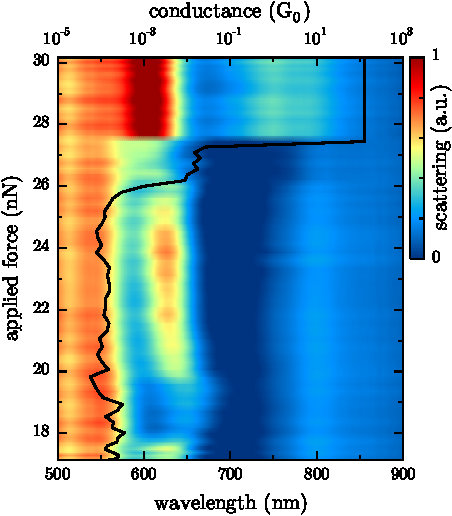
\includegraphics{figures/orig_spherical_tip_dimer_tunnelling_focus}};
\node [above right] at (0,0) {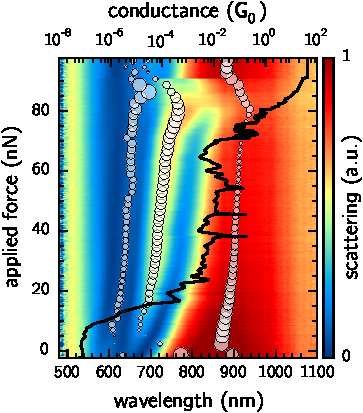
\includegraphics{figures/spherical_tip_dimer_1_tunnelling_focus}};
\node [below left] at (0,0) {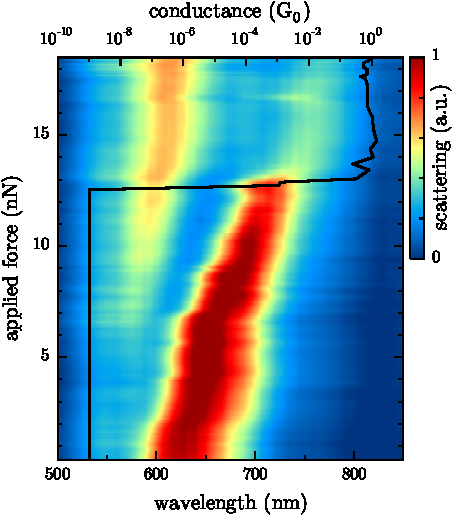
\includegraphics{figures/echem_tip_dimer_tunnelling_focus}};
%\node [below right] at (0,0) {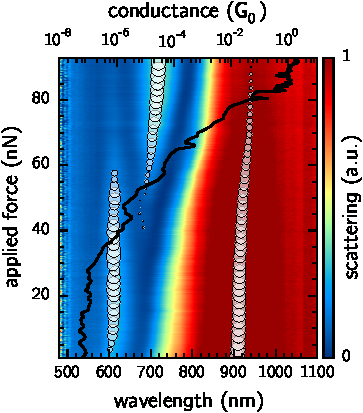
\includegraphics{figures/spherical_tip_dimer_2_tunnelling_focus}};
\node [below right] at (0,0) {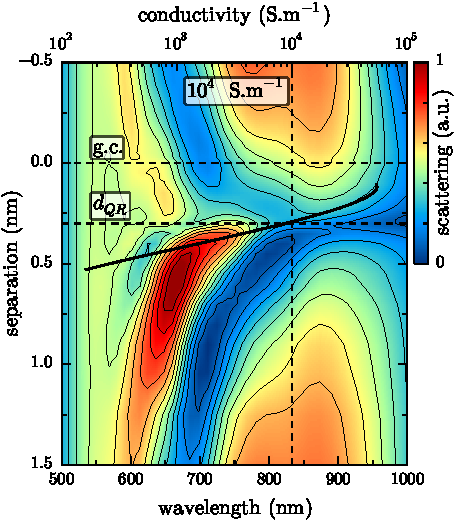
\includegraphics{figures/qcm_tip_theory_zoom_rot}};
\node at (-7.6,8.2) {\textbf{a}};
\node at (0.3,8.2) {\textbf{b}};
\node at (-7.6,-0.8) {\textbf{c}};
\node at (0.3,-0.8) {\textbf{d}};
\end{tikzpicture}
\caption[Scans of multiple spherical tip dimers passing through the quantum regime and pushing towards geometrical contact]{\textbf{Scans of multiple spherical tip dimers passing through the quantum regime and pushing towards geometrical contact.} Scans (a--c) show optical (SDF) scattering spectra as a function of the applied force on the gap with simultaneously measured conductance superimposed. The circles highlight the position of the peak with their size indicating the amplitude from a fitted model. Scans (a) and (b) use Au-coated NanoTools B150 spherical AFM probes to form a dimer while (c) uses electrochemically-fabricated AuNP-on-Pt AFM tips. Calculated QCM spectra of a spherical tip dimer as a function of separation, replotted from \cite{savage2012}, is shown in (d). Simulated spectra show both coupled modes disappearing prior to geometrical contact (g.c.) at a critical separation $d_{QR}=\SI{0.31}{nm}$, shortly followed by the rise of CTP modes. Based on DFT calculations the critical conductivity is \SI{e4}{S.m^{-1}} (\SI{0.4}{\G0.nm^{-2}}). These effects are seen in experimental scans once the conductance surpasses 2\G0.}
\label{fig:spherical_tip_scans}
\end{figure}

\autoref{fig:spherical_tip_scans} shows a selection of spherical Au tip dimer measurements showing both optical and electronic behaviour once in the sub-nm regime. Simultaneous quantum transport and SDF scattering measurements are presented as a function of the applied force compressing the gap. Each set of measurements exhibits the characteristic quantum regime transition between hybridised gap plasmons and charge transfer plasmons. However, comparison between sub-nm gaps formed in different tip dimers proves more difficult as the positions and shifts of plasmon resonances can behave very differently, regardless of any similar agreement between scans in previous coupling regimes. These differences are thought to originate from surface roughness or even smaller differences in nanoscale surface morphology that effect the way optics and electronics couple \cite{zuloaga2009, barbry2015}.%
\footnote{Changes in CTP position and intensity are said to originate from the touching profile of the dimer, indicating that the surface roughness may play a role with such large dimer surfaces \cite{zuloaga2009, barbry2015}.}

\figurenames~\ref{fig:spherical_tip_scans}a and \ref{fig:spherical_tip_scans}b bear the closest resemblance to recent theory, showing both screening and CTP formation through the quantum regime (the original QCM spectra of sub-nm gaps between spherical Au tips from \cite{savage2012} is replotted in \autoref{fig:spherical_tip_scans}d with the DFT-calculated conductivity overlaid). Experimental plasmon modes appear at similar wavelengths to QCM predictions. Screening is indicated by a reduction in the rate of redshift and a decrease in scattering intensity. A blueshifting transition between coupled plasmons and emerging CTPs signifies the rise of stronger interparticle currents. The unseen fundamental CTP is expected to exist in the IR, outside the measurable spectral range of the current microscope, though the tip's neck joint may short this mode and prevent its existence. The behaviour of hybridised modes and higher order CTPs is thus used to interpret gap behaviour.

In both experiments, the redshift of each coupled mode becomes stunted with the onset of tunnelling, revealing that the conductance has risen sufficiently to begin screening gap coupling. The point of blueshift is less clear in \autoref{fig:spherical_tip_scans}a due to the fast transition into geometrical contact. This jump is experienced in almost all scans and is attributed to a combination of the electrostatic pull between tips and a sudden decrease in mechanical resistance once the water molecules in the gap are displaced. The approach shown in \autoref{fig:spherical_tip_scans}b is much more carefully controlled going into geometrical contact and provides a much clearer insight into the origins of the blueshift. The scan is likely the single most informative scan, containing many measurements in both the tunnelling and conductive regimes, including clear observation of discretely quantised conductance channels. It is at the transition between tunnelling and ballistic conduction, at around 2\G0, that the blueshift of plasmon resonances begins to occur and tips enter the quantum conductive regime. This is in good agreement with the principles underpinning quantum theoretical models \cite{zuloaga2009}.

\begin{figure}[bt]
\centering
\begin{tikzpicture}
\node [below left] at (0,0) {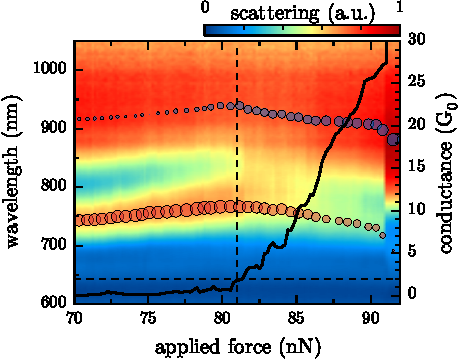
\includegraphics{figures/spherical_tip_dimer_1_tunnelling_focus2}};
\node [below right] at (0,-0.6) {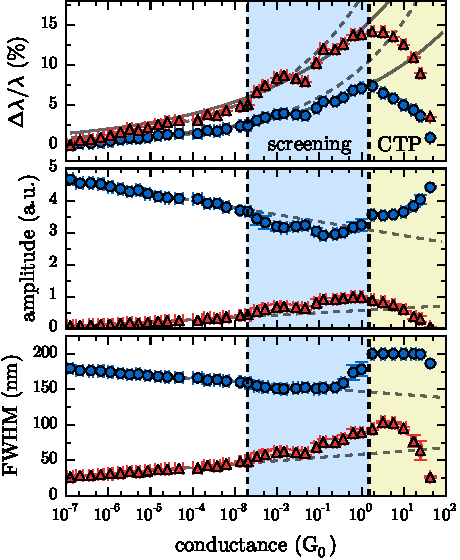
\includegraphics{figures/spherical_tip_dimer_1_tunnelling_analysis}};
\node [below left] at (-7.5,-0.5) {\textbf{a}};
\node [below right] at (0,-0.5) {\textbf{b}};
\end{tikzpicture}
\caption[Detailed analysis of a spherical Au tip dimer scan in the quantum charge transfer regime]{\textbf{Detailed analysis of a spherical Au tip dimer scan in the quantum charge transfer regime.} The scan shown in \autoref{fig:spherical_tip_scans}b is replotted in (a) with a linear conductance scale to show quantised conductance stepping and its relationship with scattering spectra. Dashed lines indicate the point of blueshift at $G=2\G0$. Peak positions in the fitted model are denoted by circles superimposed onto spectra with their size corresponding to the peak amplitude. The relative shifts, amplitudes and widths of each mode from fitted parameters are plotted in (b). Vertical dashed lines highlight the transitions into the tunnelling (crossover) regime at \num{2e-3}\G0 and the conductive regime at 1.5\G0. Exponential curves are fitted to the wavelength shift for $G<\num{e-3}\G0$ (dashed) and $G>\num{2e-3}\G0$ (solid) to highlight the reduction in redshift caused by passing through the screening (tunnelling) threshold. Similar lines are plotted to show changes in the amplitude and width upon passing through \num{2e-3}\G0.}
\label{fig:scan3_analysis}
\vspace{-5pt}
\end{figure}

A better view of this transition is shown in \autoref{fig:scan3_analysis}a with a linear conductance scale in order to closer inspect charge transfer behaviour. The turning point in the redshift of both coupled plasmons visually appears to occur at 2\G0. Fitting spectra and extracting the behaviour of each individual mode provides a more quantitative analysis. The results of the fit are superimposed onto spectra in \autoref{fig:scan3_analysis}a with fit parameters shown separately in \autoref{fig:scan3_analysis}b. Mode positions approximately follow an exponential model as expected. At \num{2e-3}\G0 the plasmon redshifts, along with their amplitudes and widths, deviate from this model and becomes less pronounced, indicating entry into the tunnelling regime of plasmonics. Prior to this point the amplitude of the lower order mode is decreasing, likely due to increasing charge localisation. Upon passing through this first critical conductance at \num{2e-3}\G0 the amplitude is further screened and decreases faster. The higher order mode continues to gain intensity at this point, potentially from redistributed charge of the lowest order mode. Similar behaviour is found in the mode widths.

The second critical conductance occurs at 2\G0, just after transitioning from tunnelling into a quantum conductive regime, i.e.\ once the Fermi level is above the gap barrier. Upon surpassing 2\G0 the resonance positions of both coupled plasmons begin to strongly blueshift into CTPs as current passes through the junction, quickly returning to their initial resonance positions prior to entering the tunnelling regime. During this transition the intensity and width of the lowest energy plasmon begins to increase, while the higher order plasmon attenuates into only a weak, blueshifted resonance. This CTP becomes fully developed during the final pull into geometrical contact. %{\color{red}A third critical conductance for CTP development is estimated to be around 10\G0 with full development between 30--40\G0.}

Despite integer quantised conductance being observed in the early conductive regime, there is no obvious step-wise shifting of plasmon resonances. It would be intuitive to expect quantised current changes to discretise incremental blueshifts, however this appears not to be the case with the blueshift appearing smooth throughout. More experimental and theoretical data would be needed to properly understand this phenomenon.

% May not be necessary
Both sets of measurements at the focus of this discussion are not without their issues, however, when compared with both theory and previous experimental results. \autoref{fig:spherical_tip_scans}a shows variations in both the position and intensity of the \SI{600}{nm} mode, which are attributed to changes in the torsional force on the gap, corresponding to a rotational motion of the tip. The mode also does not appear to shift as much as expected. The intensities of the final two modes when in contact are also reversed compared with QCM predictions. \autoref{fig:spherical_tip_scans}b looks remarkably closer to theory.

\autoref{fig:spherical_tip_scans}c shows a somewhat different phenomena to previous scans, though still in line with expectations and bearing an interesting similarity with higher order plasmons in QCM spectra. Tips in \autoref{fig:spherical_tip_scans}c are highly asymmetric AuNP-on-Pt tips, smoothed using piranha solution. Both cantilevers have \SI{40}{N.m^{-1}} spring constants, hence the force resolution during approach is limited. Prior to tunnelling a higher order mode begins to emerge. The transition into contact is quick, with few to zero points at any given conductance, ending initially with a stable 0.75--1.5\G0 contact. The initial LSP resonance quickly diminishes with the rise of the conductance without blueshifting and the higher order resonance gains intensity. The screening here is another example of entering into a tunnelling regime but without sufficient current to enter into the conductive regime and form CTPs.

\begin{figure}[bt]
\centering
\begin{tikzpicture}
\node [below left] at (0,0) {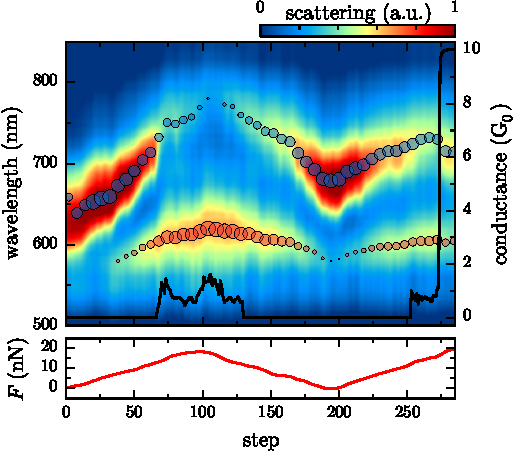
\includegraphics[width=8cm]{figures/echem_tip_dimer_tunnelling_focus_2}};
\node [below right] at (0,-0.2) {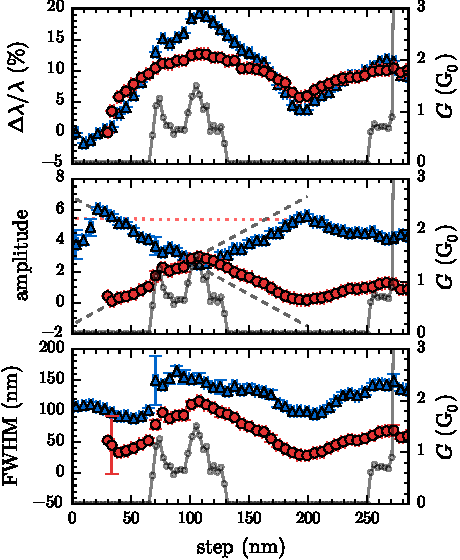
\includegraphics{figures/echem_tip_dimer_tunnelling_analysis}};
\node [below left] at (-7.7,-0.2) {\textbf{a}};
\node [below right] at (0.05,-0.2) {\textbf{b}};
\end{tikzpicture}
\caption[Detailed analysis of the extended electrochemically-fabricated spherical AuNP-on-Pt tip dimer scan]{\textbf{Detailed analysis of the extended electrochemically-fabricated spherical AuNP-on-Pt tip dimer scan.}
An extended plot of the  scan shown in \autoref{fig:spherical_tip_scans}c is plotted in (a), demonstrating reproducibility in approaches. The applied force trace represents separation changes between tips, with tips approached, retracted and then finally approached into geometrical contact. Peak positions in the fitted model are denoted by circles superimposed onto spectra with their size corresponding to the peak amplitude. The relative shifts, amplitudes and widths of each mode from fitted parameters are plotted in (b). Reduced rates of redshift are found in the $G\sim1\G0$ regions with a discontinuous blueshift seen after the $G>2\G0$ transition. Linear rates of amplitude variation are revealed from peak fits after removing the width contribution from the peak intensity. A dotted red line shows the constant sum of the amplitudes. The FWHM of each mode initially increases with conductance.}
\label{fig:echem_tip_dimer_analysis}
\end{figure}

After the initial conductance increase, the tip is immediately retracted to test for reproducibility, as shown in the extended scan plot in \autoref{fig:echem_tip_dimer_analysis}a. This is made possible by the robustness of electrochemically fabricated tips, with their solid AuNP apices. Attempting this with commercial, spherical Au tips results in the spherical apex separating from the neck due to adhesion forces. A second approach of the tip immediately after retracting out of contact demonstrates the same phenomenon until the conductance rises above 2\G0, at which point both modes blueshift. Changes in the redshift and amplitude gradient show the effects of surface morphology as retraction introduces a small degree of misalignment. This changes the conductance channels in the local electronic landscape and how they interact with the plasmon field.

A detailed mode analysis of plasmon resonances is shown in \autoref{fig:echem_tip_dimer_analysis}b. Shifting of plasmon resonances behaves as expected. Upon increasing the conductance up to the 1\G0 level there is a visible reduction in the rate of redshift caused by screening. Once the conductance abruptly rises above 2\G0 in the second approach there is a clear blueshift in the lowest order mode, alluding to a similar critical conductance. An interesting feature in this instance is that the extracted amplitude of the initial mode linearly decreases during approach at exactly the same rate as the new mode emerges. In a sense, charge is conserved and simply switches to a more favourable mode as the gap width decreases and tunnelling rate increases.

To summarise, each of the presented three scans shows agreement with recent theoretical concepts that predict the effects of quantum mechanical charge transfer on plasmon coupling. Four different plasmonic regimes related to charge transfer can be identified: classical coupling in the absence of charge transfer, a quantum tunnelling regime, a quantum (ballistic) conductive regime and, finally, a classical conductive regime. Tunnelling is responsible for screening whereas conductive contact leads to the progressive formation of CTPs. Critical conductances for entering the tunnelling regime and the quantum conductive regime are observed in each case in the vicinity of \num{2e-3}\G0 and 2\G0, respectively. This is the first time conductance values have been experimentally correlated with optical spectra using a dynamic approach to plasmon coupling.

Critical conductances are expected to hold outside of the quantum regime similar to the previously defined screening and CTP conductance thresholds \cite{perez2010, perez2011}. Comparison with previously explored systems shows excellent agreement, supporting the idea of critical conductances. Blueshifts of the BDP, forming the SBDP, begin to be seen in small 2\G0 conductive contacts in both theoretical models \cite{perez2010, perez2011} and experimental NPoM systems when AuNPs are separated from a Au mirror by a blended SAM of variable conductance \cite{benz2014}. Observation of the same threshold conductance in two very different experimental systems provides strong evidence for the fundamental nature of critical conductances.
%Variations in measured quantum transport phenomena between tip dimers are highly likely to be the result of surface roughness changing the charge distribution on gap surfaces. In each situation plasmon coupling would behave differently depending on the localisation of field in the gap and the location and summation of all points of optical tunnelling \cite{barbry2015}.
Using this information, the plasmonics of a sub-nm plasmon system can begin to be better characterised and quantified with the aim to finally exploit plasmonics to measure optical conductivities.

\end{document}